\begin{center}
%\textit{by A. Bethani, A. Betti, P. Bokan, E. Carquin Lopez, M. Donadelli, A. Ferrari, K. Grimm, C.Gwilliam, M. Haacke, S. Lai, K.J.C. Leney, T. Lenz, S. Olivares, E. Petit, N. P. Readioff,P. Sales de Bruin, J. Stark, F. Walls, D. Wardrope, M. Wielers}
\textit{written by E. Petit, results from the ATLAS collaboration.}


\end{center}

A direct measurement of the Higgs boson trilinear self-coupling \lHHH\ can be made via the study of Higgs boson pair production. %Only the dominant production mechanism at hadron colliders, gluon fusion, is considered, with the other production mechanisms being more than an order magnitude smaller.
%The Feyman diagram which exhibits a \lHHH\ dependence interferes destructively with the box diagram that is independent of \lHHH, thus a small increase in the value of \lHHH decreases the expected HH production cross section, and modifies the distributions of event kinematics.

The small SM non-resonant HH production cross section means that it is necessary to consider final states where at least one of the two Higgs bosons decays into a final state with a large branching ratio, ie $H \rightarrow b\bar{b}$. The most promising decays channels are $HH \rightarrow b\bar{b}b\bar{b}$, $HH \rightarrow b\bar{b}\tau\tau$ and $HH \rightarrow b\bar{b}\gamma\gamma$ with branching ratios of 33.9, 7.3 and 0.26\% respectively.

The expected performance for the $b\bar{b}b\bar{b}$ and $b\bar{b}\tau\tau$ channels is assessed through extrapolation of measurements performed by the ATLAS detector using 24.3~\fbinv\ and 36.1~\fbinv\ of data, respectively, obtained at $\sqrt{s} = 13$~\TeV\ during Run 2.
The expected performance for the $b\bar{b}\gamma\gamma$ channel is assessed through the use of truth-level Monte Carlo samples. 
These MC samples have been adjusted with parametrised functions to estimate the response of the upgraded ATLAS detector at the HL-LHC, assuming a mean pile-up rate <$\mu$> = 200. 
An 8\% improvement in b-tagging efficiency is expected for all channels as a result of improvements to the inner tracker~\cite{ITKPixelTDR}.
This improvement is factored into the $b\bar{b}b\bar{b}$ and $b\bar{b}\tau\tau$ extrapolations, and it is included in the smearing functions used in the $b\bar{b}\gamma\gamma$ analysis.

A short description of the analysis strategy and of the results is given here, and further details can be found in Ref.~\cite{ATLASHHPUBnote}. The systematic uncertainties used follow the common recommendations for HL-LHC studies~\cite{ATLASperfPUBnote}. 



%
\paragraph{The $HH \rightarrow b\bar{b}b\bar{b}$ channel}

Projections for this channel were made by extrapolating from the ATLAS Run 2 analysis of 24.3 \fbinv\ of 13~\TeV\ data, described in Ref.~\cite{ITKPixelTDR}. This extrapolation assumes similar detector performance to Run~2. Four central jets with transverse momentum higher than 40~\GeV\ are paired to construct the Higgs boson candidates. Additional requirements are made on Higgs boson mass and transverse momentum, and the pseudorapidity between the two Higgs boson candidates.
The acceptance times efficiency of the full event selection for the SM signal is of 1.6\%, and around 95\% of the background consists of multi-jet events. This dominant background is assessed using data-driven techniques. 

The largest source of systematic uncertainty comes from the ability to model the QCD multi-jet background using control regions in data. A conservative assumption in the extrapolation is made that the systematic uncertainties related to this background are left unchanged. Figure~\ref{fig:ATLAS_HH_4b_a} shows the impact of this uncertainty on the results.


\begin{figure}[!htb]
\centering 
\subfloat[]{\label{fig:ATLAS_HH_4b_a}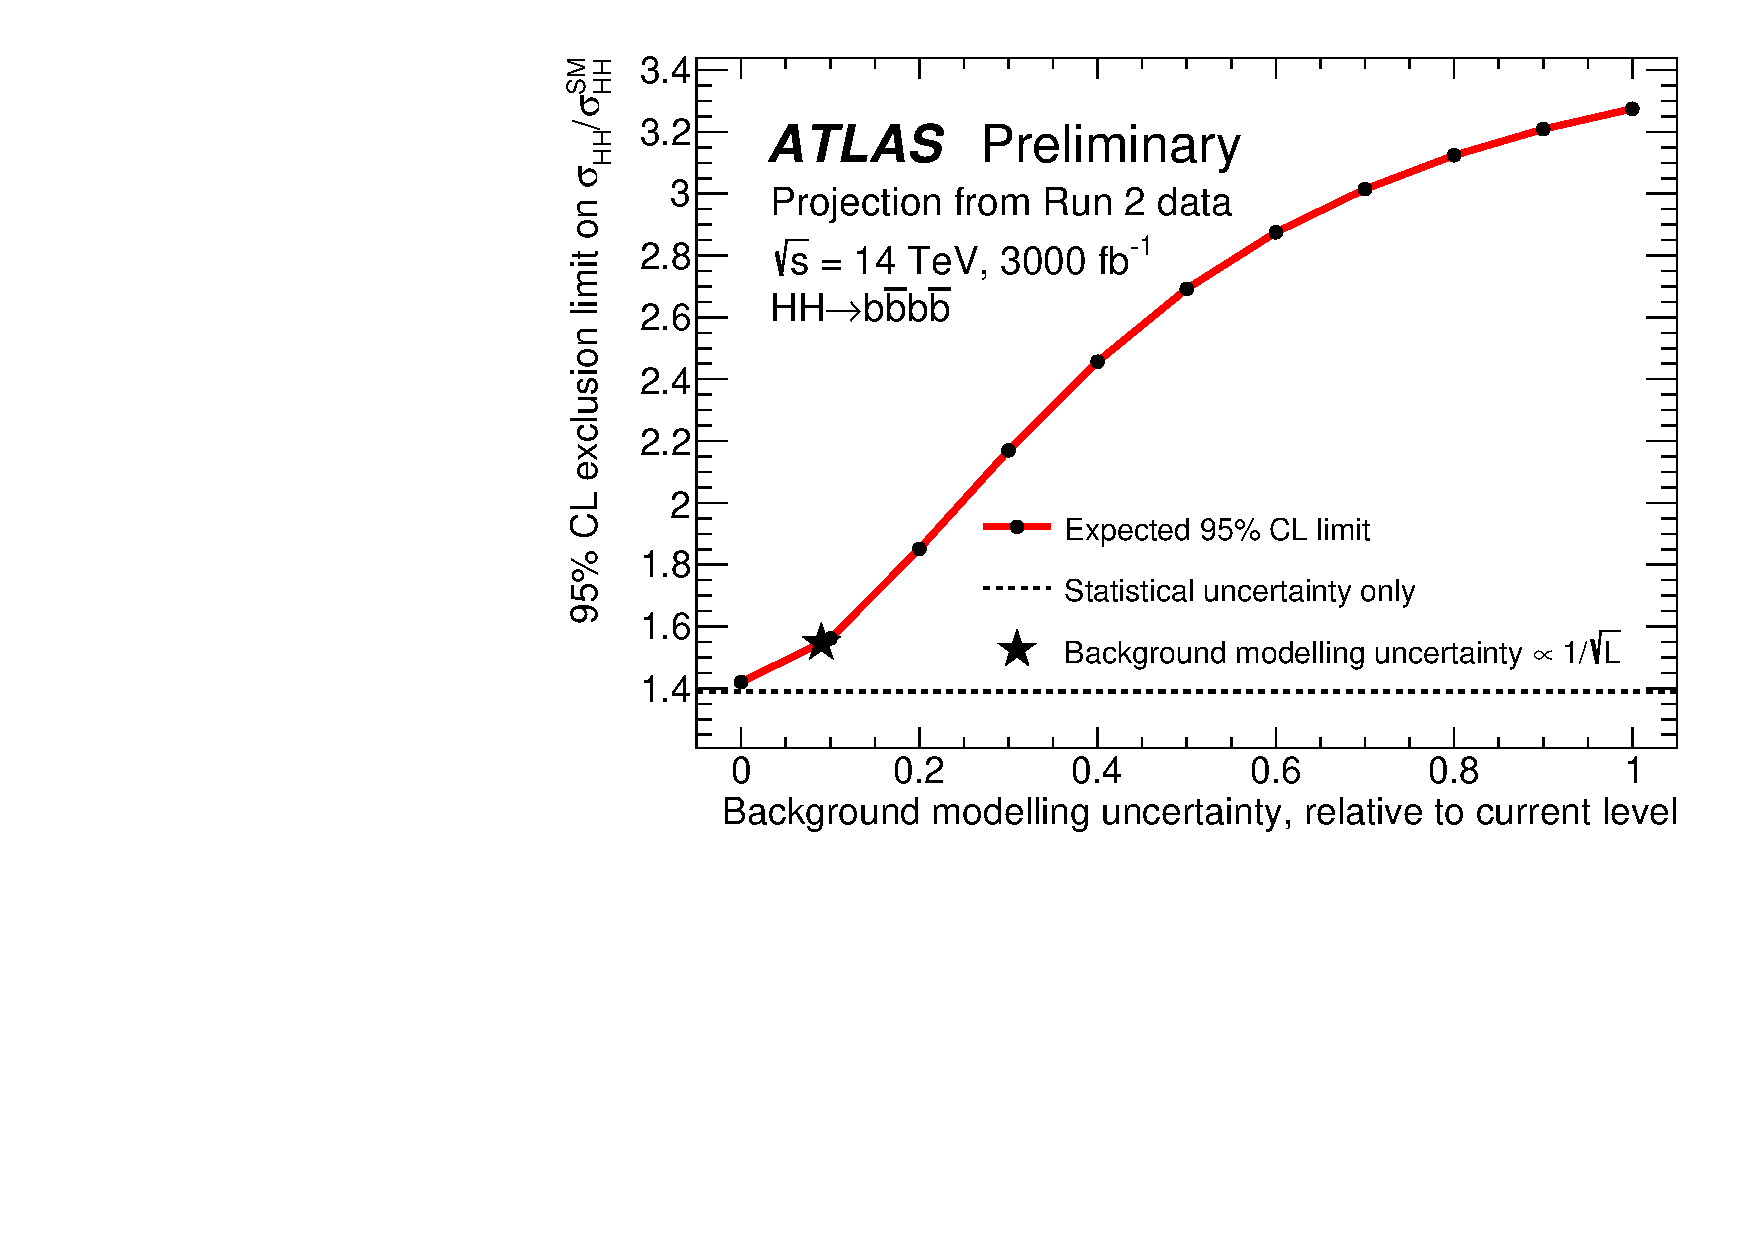
\includegraphics[width=0.5\textwidth]{\main/section3/plots/ATLAS_LimitVsSyst_Preliminary.pdf}} 
\subfloat[]{\label{fig:ATLAS_HH_4b_b}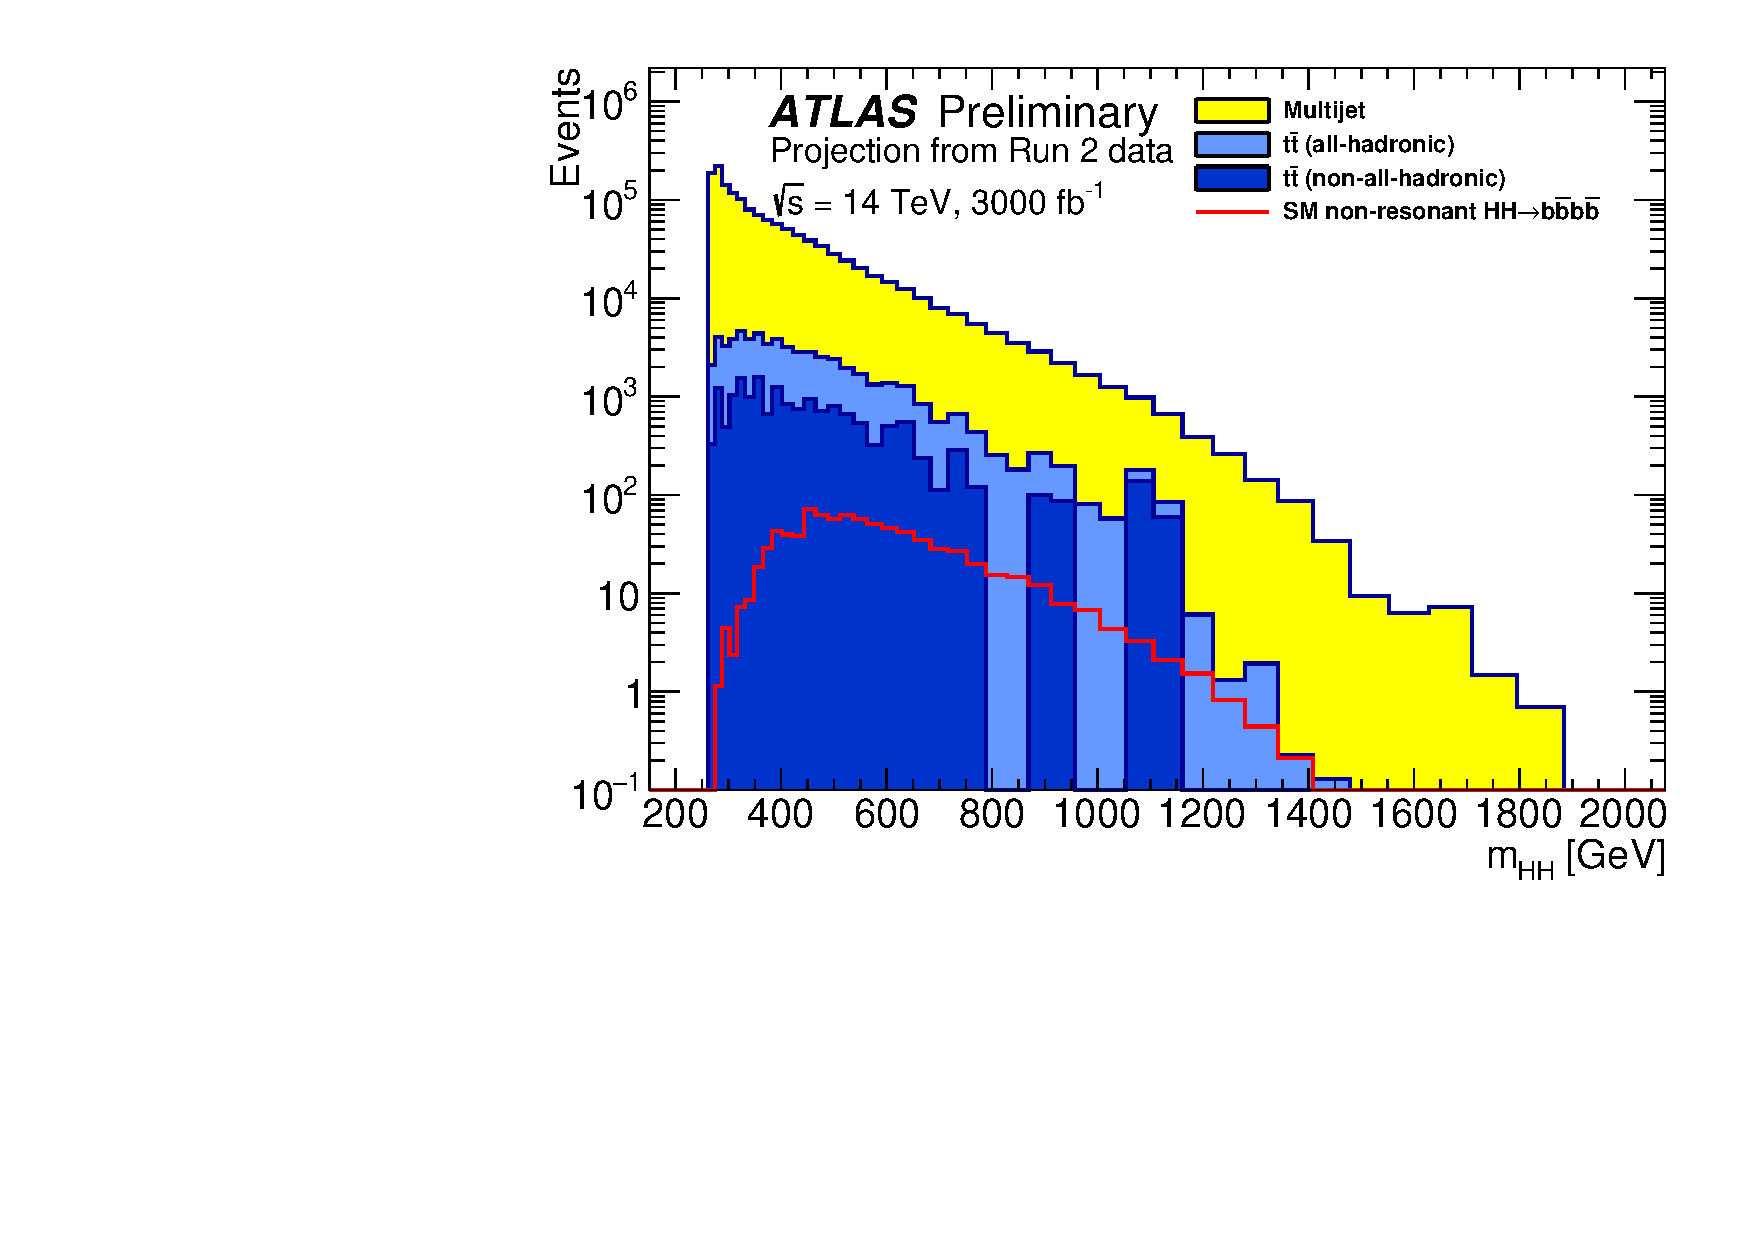
\includegraphics[width=0.5\textwidth]{\main/section3/plots/M4jDistribution_3000fb_Preliminary.pdf}}
\caption{(a) Expected 95\% CL upper limit on $\sigma_{HH}/\sigma_{HH}^{SM}$, as a function of the pre-fit background modelling uncertainties, which are each scaled by a common, constant factor relative to the corresponding uncertainty in the Run~2 analysis (i.e. the uncertainties of the analysis of the 2016 dataset correspond to 1 here). 
The limit achievable assuming that the overall uncertainty scales with luminosity as $1/\sqrt L$ is shown by the star point.
The limit obtained when considering only statistical uncertainties is shown as the dashed line.
The extrapolated sensitivities are calculated assuming a jet \pt\ threshold of 40 \GeV.
(b) Stacked $m_{HH}$ histograms of the \ttbar\ and multi-jet backgrounds extrapolated from 24.3~\fbinv\ (the 2016 dataset) to 3000~\fbinv.
The predicted SM non-resonant Higgs boson pair production signal is shown as the red line.} 
\label{fig:ATLAS_HH_4b} 
\end{figure}

The final analysis discriminant, m$_{HH}$, showed in Figure~\ref{fig:ATLAS_HH_4b_b}, is the invariant mass of the selected four-jet system, after a correction based on the known Higgs boson mass. The significance neglecting the systematic uncertainties is 1.4 standard deviations, while it is 0.61 standard deviations when the current systematic uncertainties are included. 
The high number of pile-up events at the HL-LHC cause difficulties in maintaining high acceptance when triggering on multi-jet final states. Ref.~\cite{Collaboration:2285584} proposes a trigger menu which thresholds corresponding to asking for jets with a transverse energy higher than 75~\GeV. In the scenario without systematic uncertainties this would degrades the sensitivity by 50\% relative to the threshold used by default in this extrapolation.

%The allowed range at 95\% CL for $\kl$ including (without) systematic uncertainties is -4.1 -- 8.7 (-1.2 -- 8.0).

%
\paragraph{The $HH \rightarrow b\bar{b}\tau\tau$ channel}

Results~\cite{ATLASHHPUBnote} for this channel are computed by extrapolating from the Run 2 analysis of 36.1~\fbinv\ of 13~\TeV\ data~\cite{ATLASrun2HHbbtautau}, which currently sets the world's strongest limit by a single channel on the di-Higgs production. 
The leptonic/hadronic and hadronic/hadronic decay modes of the $\tau$-lepton are considered, the first one being separated in two categories, depending on the trigger used. A multivariate analysis with a Boosted Decision Tree is performed to separate the signal from the background processes. The Run~2 BDT distributions are scaled to the integrated luminosity of 3000~\fbinv, taking into account the change of cross-section with the increased centre-of-mass energy. The binning of those BDT distributions is also redefined to take into account the increased number of events.
A profile-likelihood fit is applied to the BDT score distributions shown in Figures~\ref{fig:ATLAS_HH_bbtautau_a} to~\ref{fig:ATLAS_HH_bbtautau_c}. 


\begin{figure}[!htb]
\centering 
\subfloat[$\tau_{lep}\tau_{had}$ channel passing a single-lepton trigger (SLT)]{\label{fig:ATLAS_HH_bbtautau_a}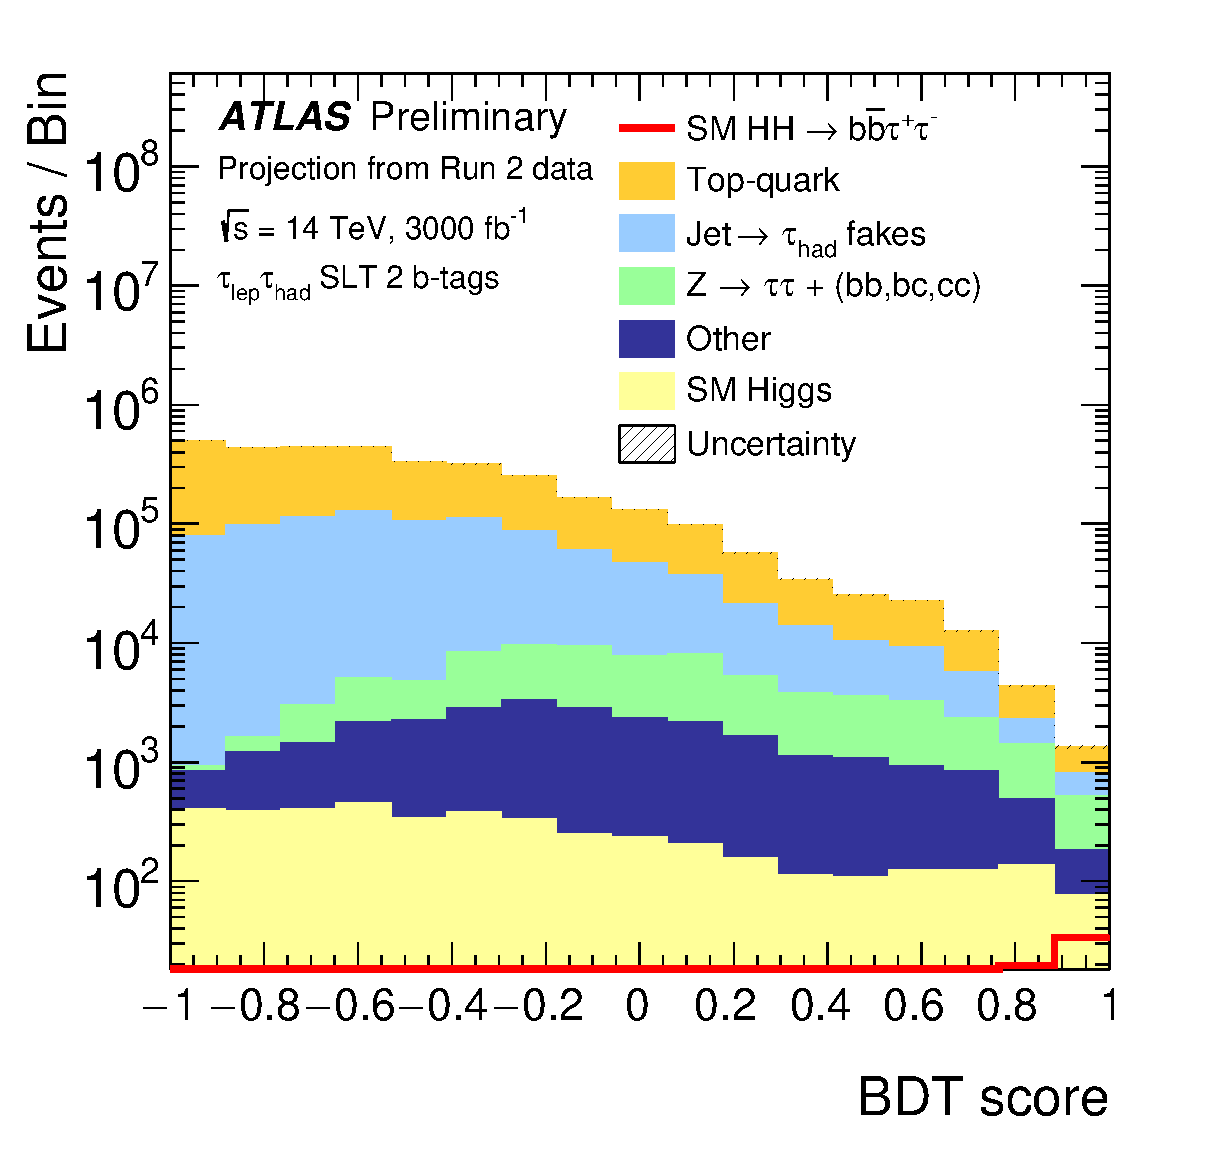
\includegraphics[width=0.5\textwidth]{\main/section3/plots/TauLH_SLT_BDTScore}} 
\subfloat[$\tau_{lep}\tau_{had}$ channel passing a lepton-plus-$\tau_{had}$ trigger (LTT)]{\label{fig:ATLAS_HH_bbtautau_b}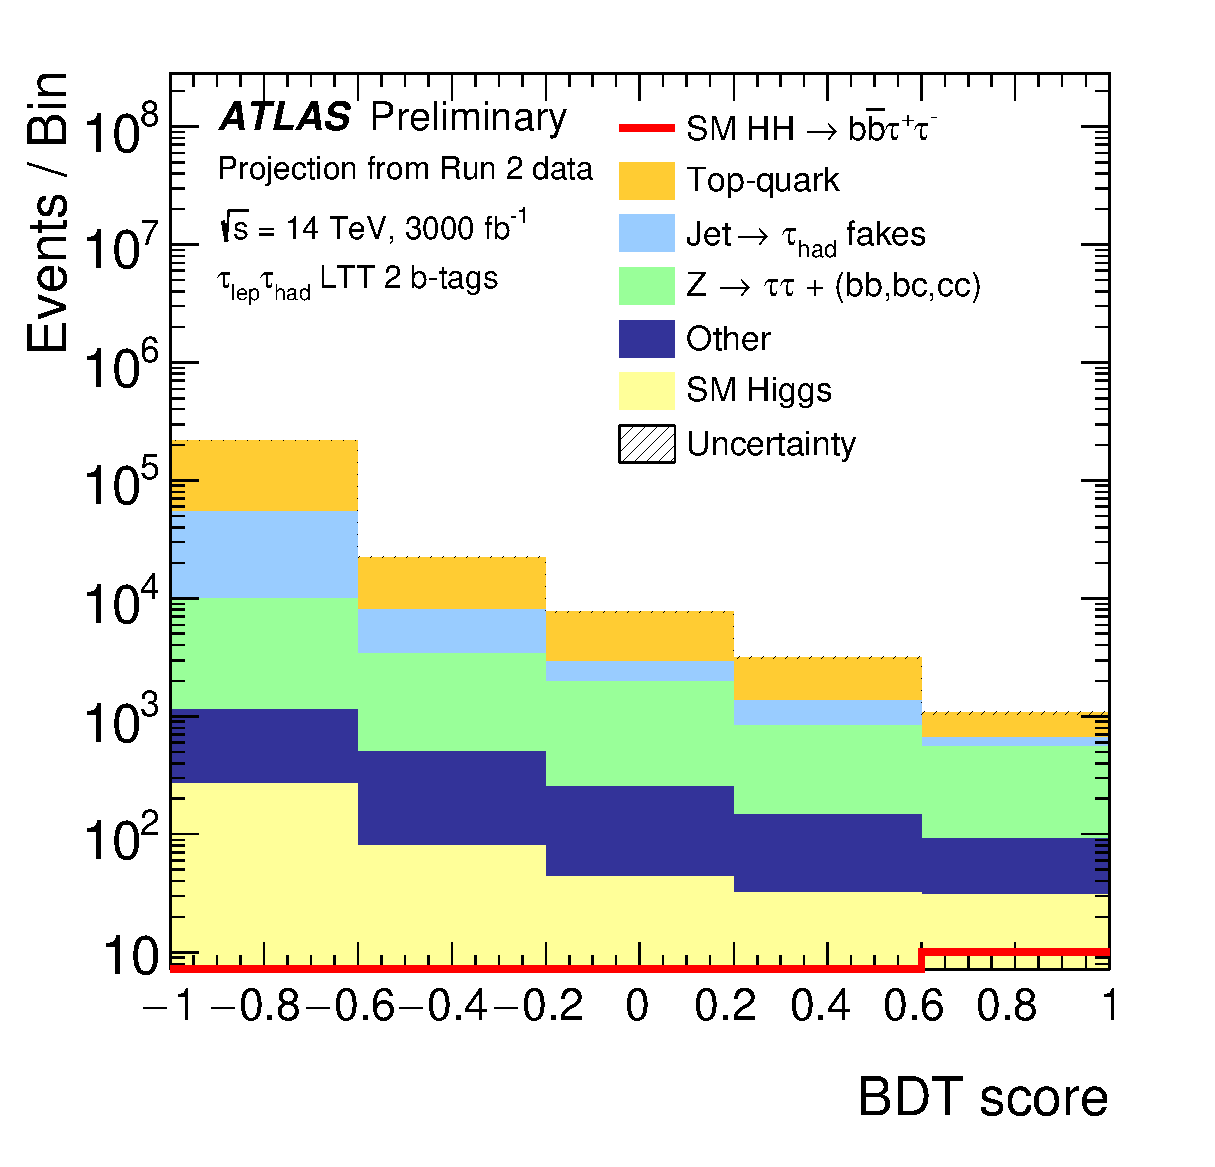
\includegraphics[width=0.5\textwidth]{\main/section3/plots/TauLH_LTT_BDTScore}}\\
\subfloat[$\tau_{had}\tau_{had}$ channel]{\label{fig:ATLAS_HH_bbtautau_c}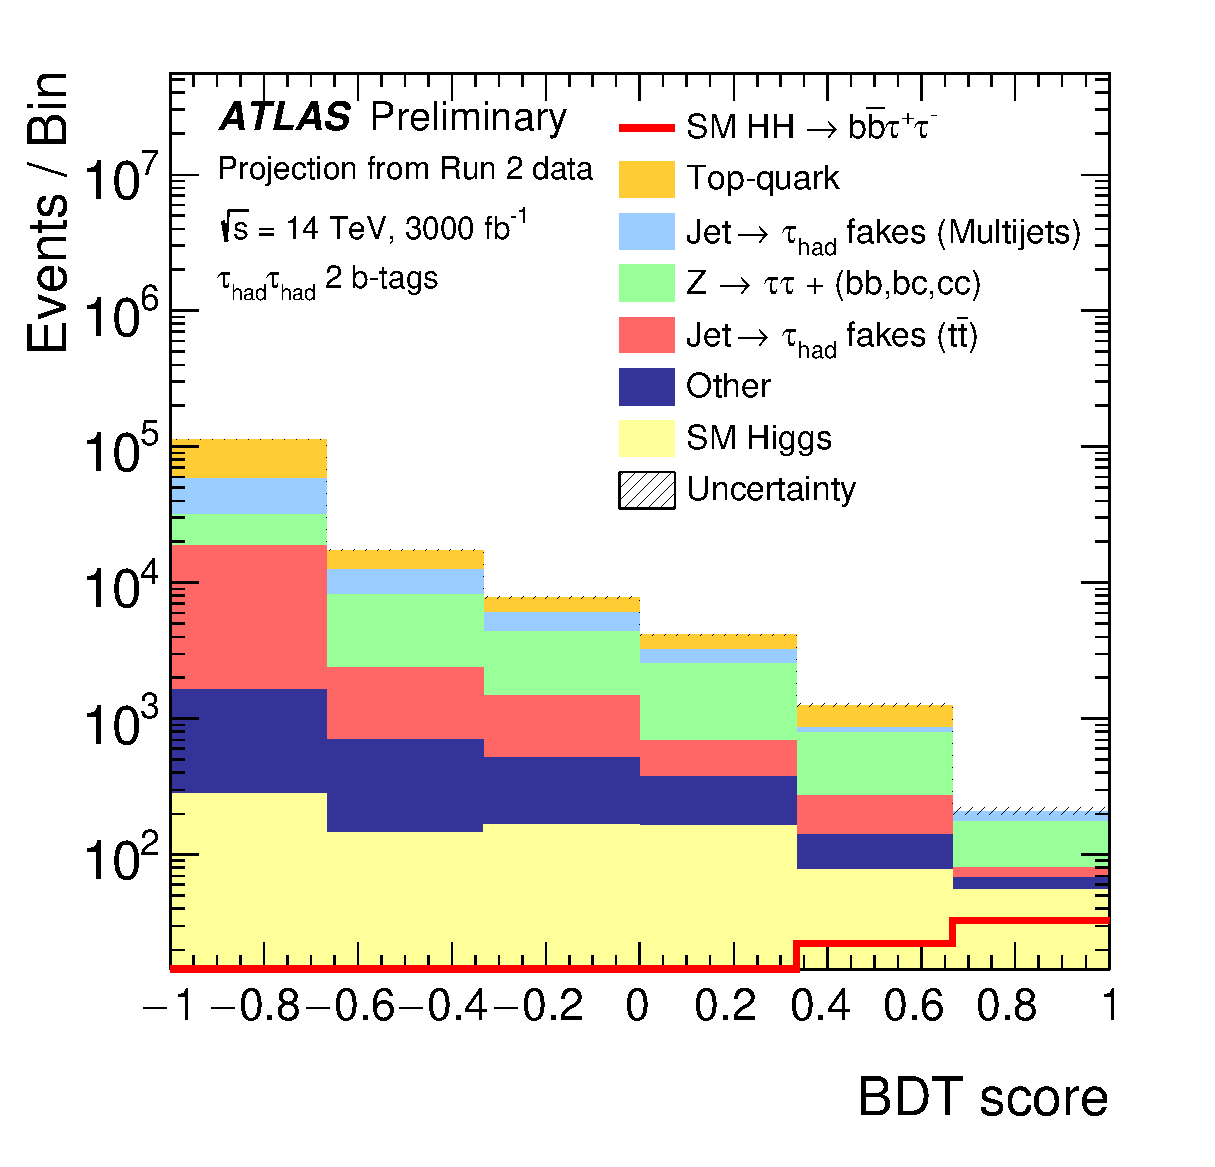
\includegraphics[width=0.5\textwidth]{\main/section3/plots/TauHH_BDTScore}}
\subfloat[]{\label{fig:ATLAS_HH_bbtautau_d}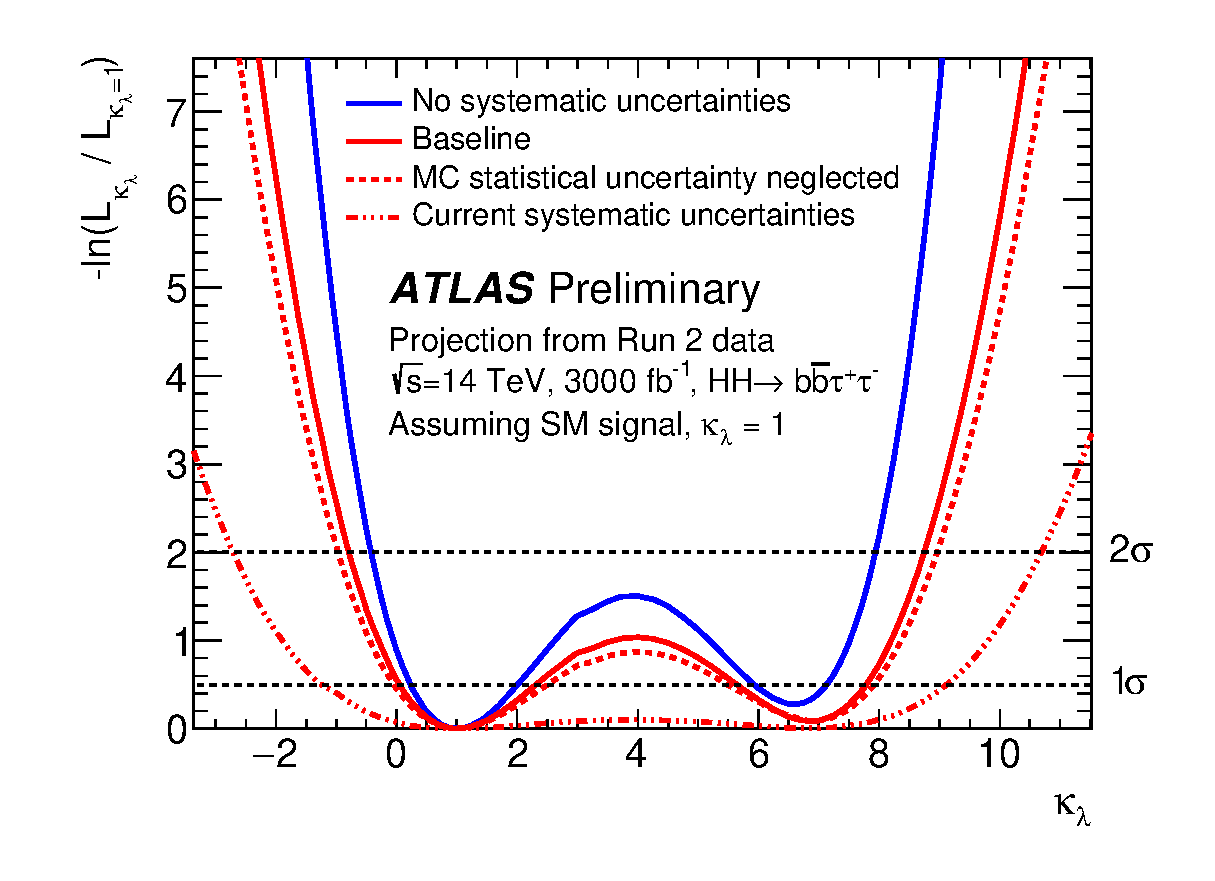
\includegraphics[width=0.5\textwidth]{\main/section3/plots/delta_NLLnew4_tautau_Systs_ApprovedRWbeffXsecFixedSMinj_TauTau_3000_Final1909StatOnlySMinjTT3000}}
\caption{(a), (b), (c) Distributions of the BDT score for the three categories of the analysis, extrapolated to 3000~\fbinv\ of data. The background distributions are shown after the fit based on a background-only Asimov dataset and the signal is scaled to the SM prediction. The hatched bands represent the combined statistical and systematic uncertainty for the baseline scenario. These uncertainty bands are included in the plots for completeness but are very small. (d) Negative natural logarithm of the ratio of the maximum likelihood for $\kappa_{\lambda}$ to the maximum likelihood for $\kappa_{\lambda}$ = 1, obtained from fits to the Asimov dataset that contains the $\kappa_{\lambda}$ = 1 signal. Four different scenarios are considered for the systematic uncertainties.} 
\label{fig:ATLAS_HH_bbtautau} 
\end{figure}

In the Run~2 analysis one of the dominant systematic uncertainty is the one coming from the limited statistics of the MC samples used to estimate the background. In the baseline scenario, following the prescriptions of Ref.~\cite{ATLASperfPUBnote}, this uncertainty is neglected.
Different scenarios are considered: the one in which the systematic uncertainties remain the same as for the Run~2 analysis (scenario S1 described in Section~\ref{sec:HiggsExtrapAss}); the scenario with the current systematic uncertainties but neglected MC statistical uncertainties and the baseline scenario for systematic uncertainties (scenario S2 described in Section~\ref{sec:HiggsExtrapAss}). The effect on those various scenarios is shown in Figure~\ref{fig:ATLAS_HH_bbtautau_d}.

The expected significance without systematic uncertainties is of 2.5 standard deviations, while it is 2.1 standard deviations when the baseline scenario for the systematic uncertainties is considered.

For the measurement of \kl\ the output score of a BDT trained on the \kl\ = 20 signal is used as the final discriminant. This was shown to provide similar performance with BDTs trained specifically for every \kl\ value, as \kl\ = 20 corresponds to a softer m$_{HH}$ spectrum, which is where the nominal BDT is less sensitive.
The minimum negative-log-likelihood for a SM signal hypothesis is shown in Figure~\ref{fig:ATLAS_HH_bbtautau_d}.


%A multivariate analysis with a boosted decision tree (BDT) is performed on the leptonic/hadronic and hadronic/hadronic decay modes of the $\tau$-lepton, and the BDT score is used as final discriminant. The largest systematic uncertainty of the Run 2 analysis, the simulation statistics, is neglected in the extrapolation. The expected significance of XX (XX) $\sigma$ including (without) systematics uncertainties can be achieved. The allowed range at 95\% CL for $\kl$ including (without) systematic uncertainties is XX -- XX (XX -- XX).


%
\paragraph{The $HH \rightarrow b\bar{b}\gamma\gamma$ channel}


The analysis~\cite{ATLASHHPUBnote} is based on truth level particles convoluted with the detector resolution, efficiencies and fake rates computed for $\mu$ = 200 which were extracted from fully simulated samples using the detector layout described in Ref.~\cite{ITKPixelTDR}. The selection is made using a multivariate analysis with a BDT using the full kinematic information of the event, in particular to reject the continuum and \ttH\ backgrounds. 
The di-photon invariant mass distribution, $\ensuremath{m_{\gamma\gamma}}$, is shown in Figure~\ref{fig:ATLAS_HH_bbyy_a}. The number of signal, single Higgs and continuum background in a 123-127~\GeV\ window is 6.5, 3.2 and 3.7 respectively.

The systematic uncertainties follow the prescriptions of Ref.~\cite{ATLASperfPUBnote}. Their effect is very small since this channel will still be dominated by statistical uncertainties at the end of the HL-LHC programme.


The sensitivity of the analysis to \kl\ is assessed by using the $\mhh$ distribution for events in a 123 $ < \ensuremath{m_{\gamma\gamma}} $< 127~\GeV. This distribution is shown in Figure~\ref{fig:ATLAS_HH_bbyy_b} for different values of \kl\ and split into eight categories. It should be noted that the BDT was trained on the SM signal only, so the constraints on \kl\ are pessimistic. Using separate BDTs trained on specific values of \kl\ would bring negligible improvements at negative values of \kl, but up to 1$\sigma$ reduction in the expected limit at high positive values of \kl.
The expected significance was evaluated to be 2.1 and 2.0 standard deviations with and without systematic uncertainties included.

%The diphoton invariant mass distribution, used to extract the signal through an analytical fit, is shown in Figure~\ref{fig:ATLAS_HH_a}. The number of signal, single Higgs and continuum background in a 123-127~\GeV\ window is XX, XX and XX respectively, leading to a significance of XX (XX)$\sigma$ including (without) systematics uncertainties. The allowed range at 95\% CL for $\kl$ including (without) systematic uncertainties is XX -- XX (XX -- XX).


\begin{figure}[!htb]
\centering 
\subfloat[]{\label{fig:ATLAS_HH_bbyy_a}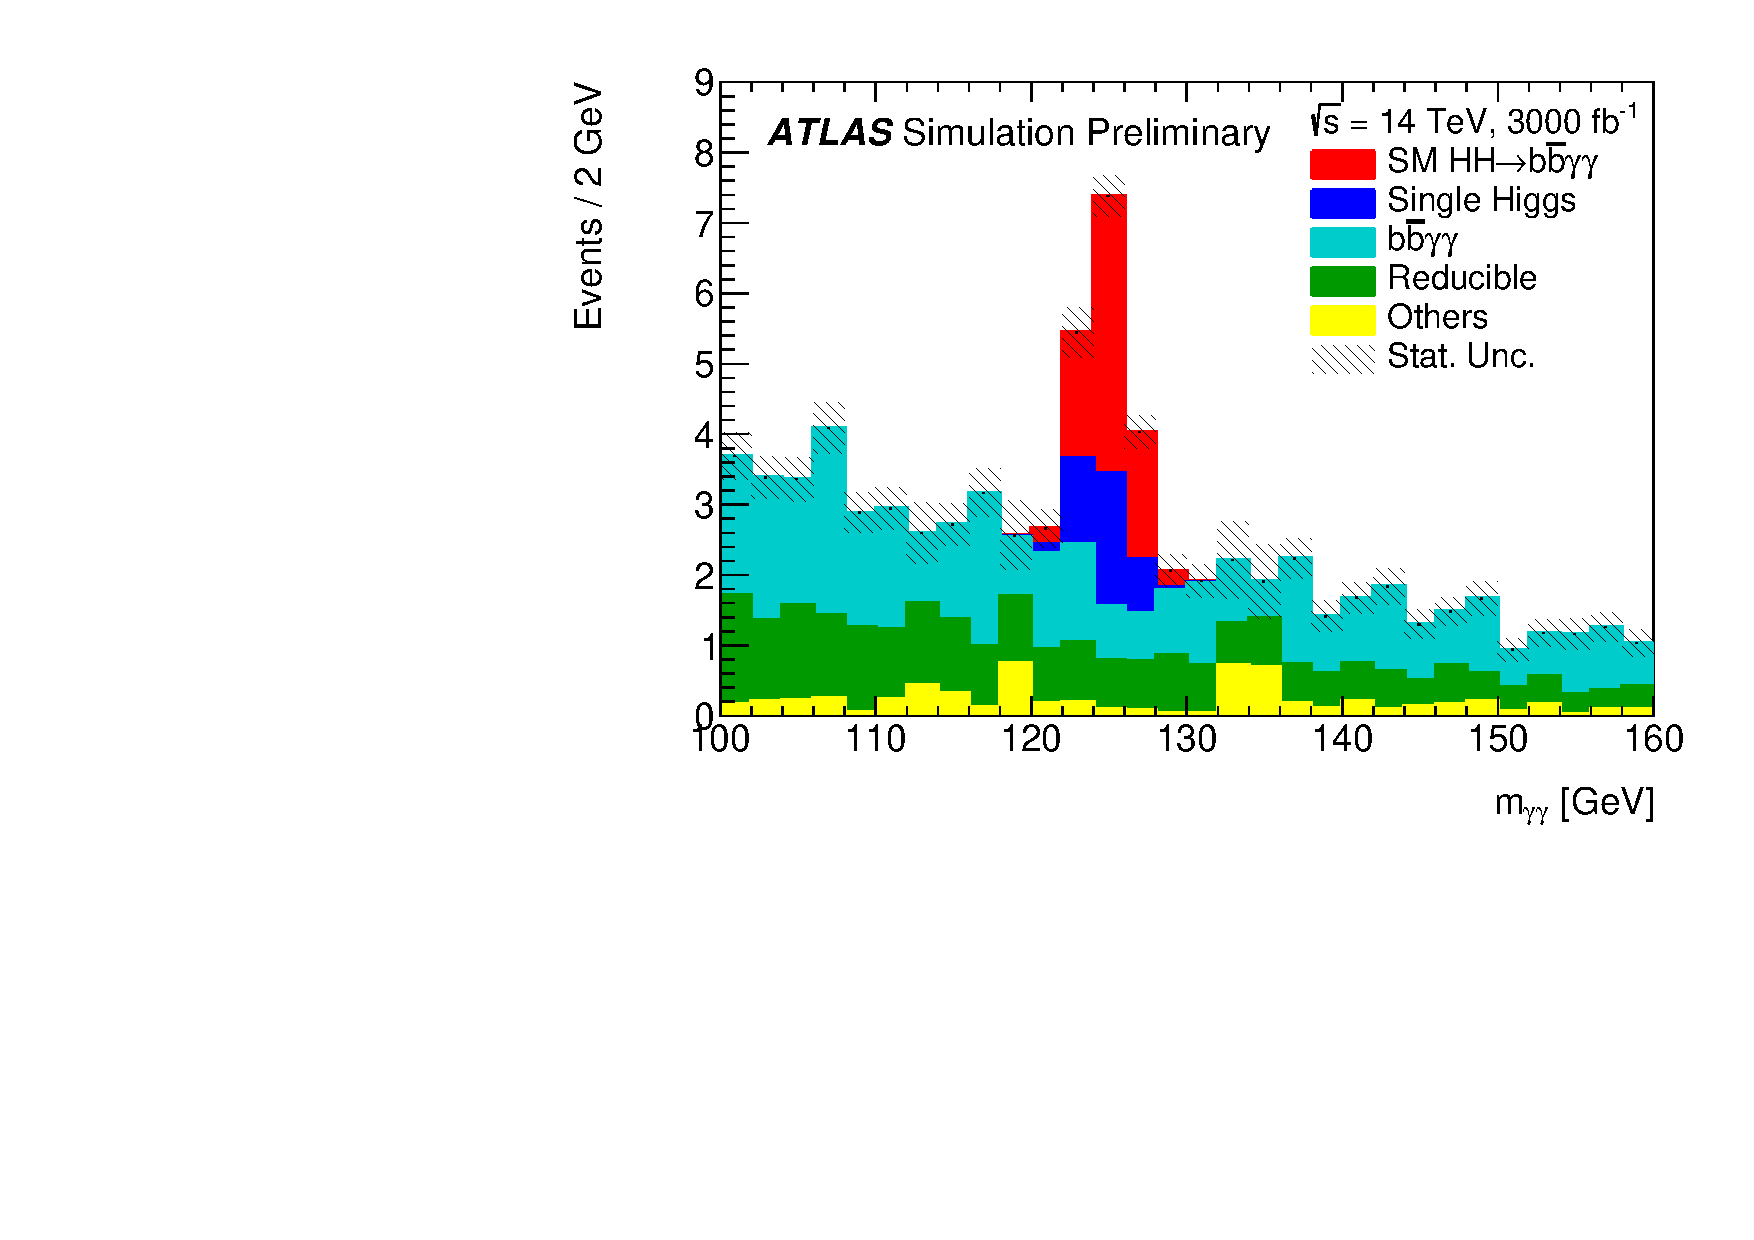
\includegraphics[width=0.5\textwidth]{\main/section3/plots/bbyy_myy_SignalBackground_2GeVbins_Preliminary}} 
\subfloat[]{\label{fig:ATLAS_HH_bbyy_b}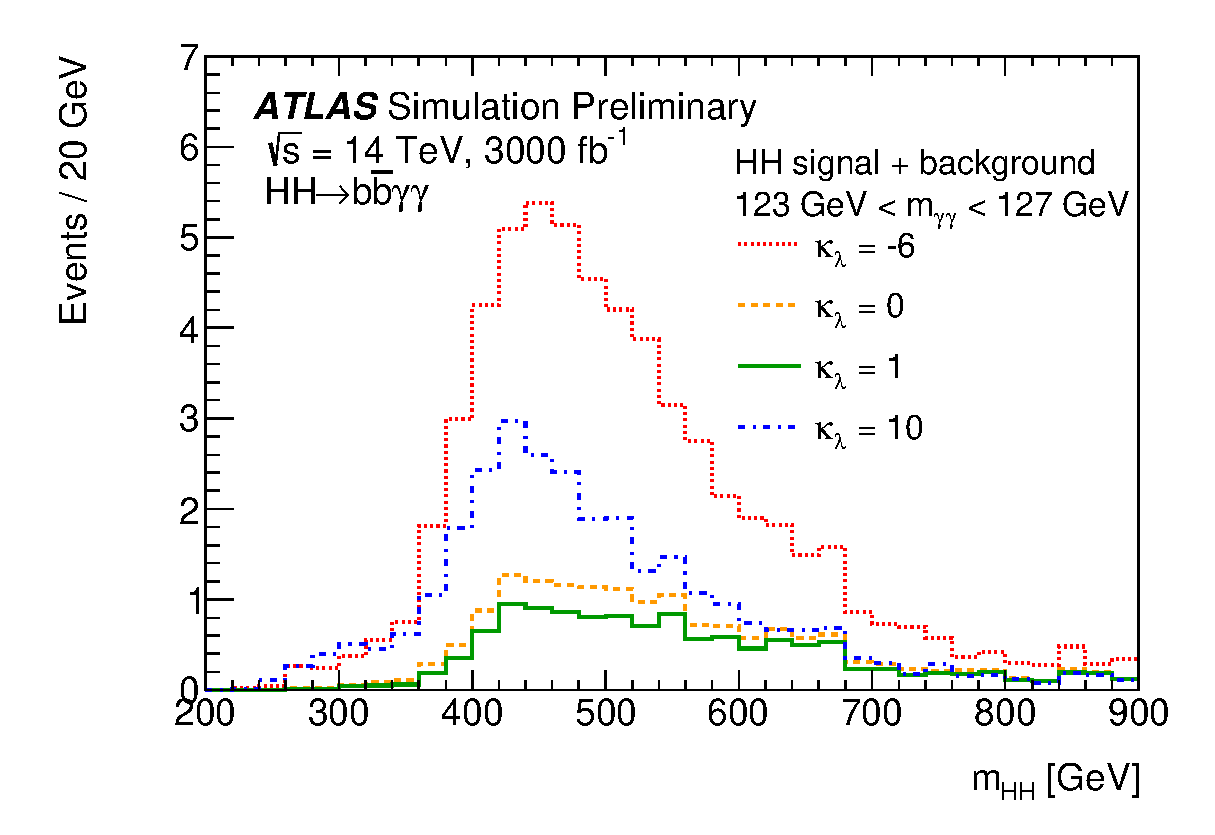
\includegraphics[width=0.5\textwidth]{\main/section3/plots/mbbyy_SignalBackground_20GeVbins_variouskappa_Preliminary}} 
\caption{(a) Distribution of $m_{\gamma\gamma}$ following the BDT response cut. The reducible background processes consist of $c\bar{c}\gamma\gamma$, $jj\gamma\gamma$, $b\bar{b}j\gamma$, $c\bar{c}j\gamma$, and $b\bar{b}jj$ events.  Other background processes come from $Z(b\bar{b})\gamma\gamma$, $t\bar{t}$ and $t\bar{t}\gamma$.
(b) Distributions of $m_{b\bar{b}\gamma\gamma}$ for combined signal and background events passing the BDT selection and the requirement 123 \GeV $ < \ensuremath{m_{\gamma\gamma}} $< 127~\GeV, for various values of $\kappa_{\lambda}$.} 
\label{fig:ATLAS_HH_bbyy} 
\end{figure}


%
\paragraph{Combined results}


The combination of various channels is realised by constructing a combined likelihood function that takes into account data, models and correlated systematic uncertainties from all channels. 

Setting appropriate nuisance parameters (NP) to be correlated with one another induced a negligible change in the combination results compared to assuming all nuisance parameters are uncorrelated. No strong correlation between any of the NP are found by the fits, with the exception of some correlation between the background models of the $b\bar{b}b\bar{b}$ and $b\bar{b}\tau\tau$ channels. Theoretical uncertainties on the cross-sections have negligible impact on the combined results.

The combined significance is 3.5 and 3.0 standard deviations with and without systematic uncertainties included.

The combined sensitivity of the three channels to \kl\ is assessed by generating an Asimov dataset containing the background plus SM signal. The ratio of the negative-log-likelihood of the maximum likelihood fit for \kl\ was calculated and shown in Figure~\ref{fig:ATLAS_HH_comb}. A morphing technique~\cite{ATL-PHYS-PUB-2015-047} is used to generate signal distributions of m$_{HH}$ for any arbitrary value of \kl.

\begin{figure}[!htb]
\centering 
\subfloat[Statistical uncertainties only]{\label{fig:ATLAS_HH_comb_a}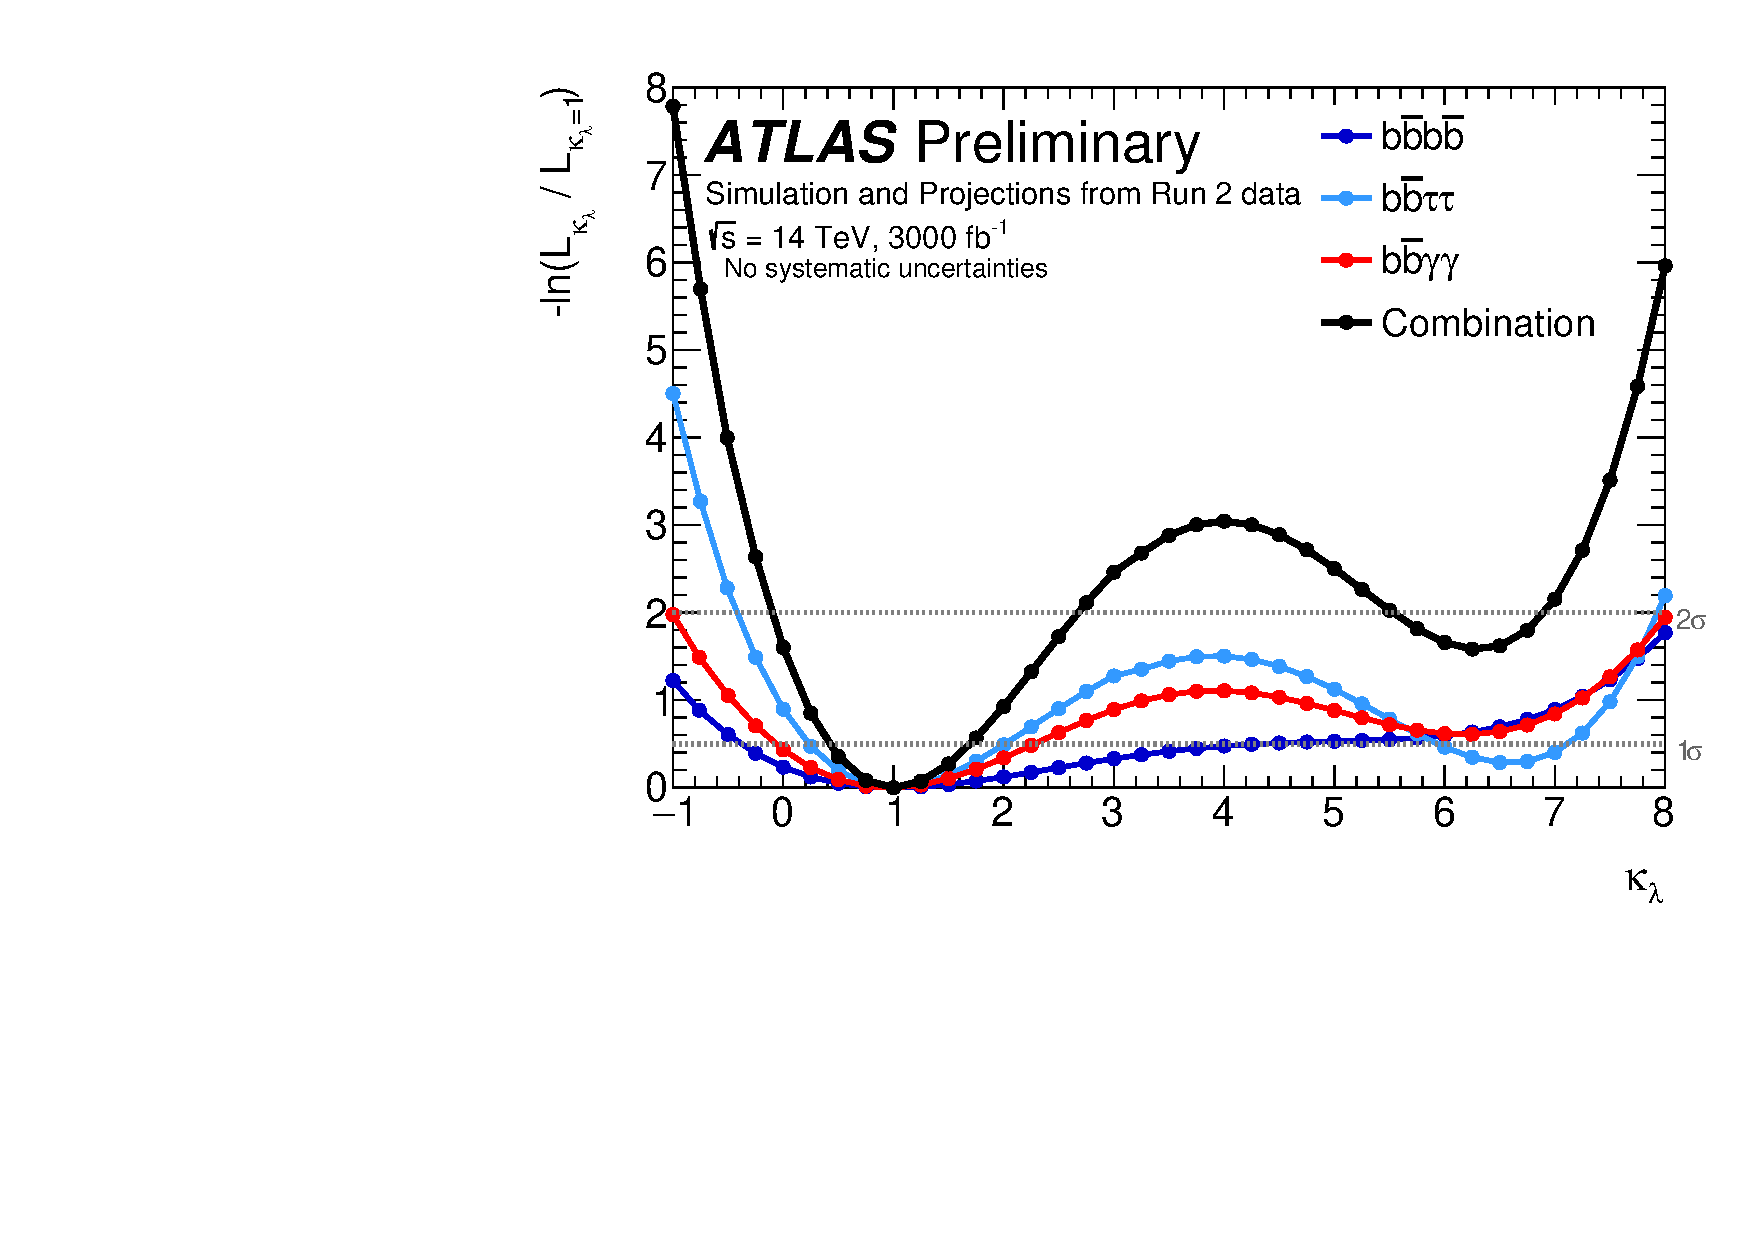
\includegraphics[width=0.5\textwidth]{\main/section3/plots/bbbb_bbtt_bbyy_lHHH0100_NoSyst_overlay_Preliminary.pdf}} 
\subfloat[Statistical + systematic uncertainties]{\label{fig:ATLAS_HH_comb_b}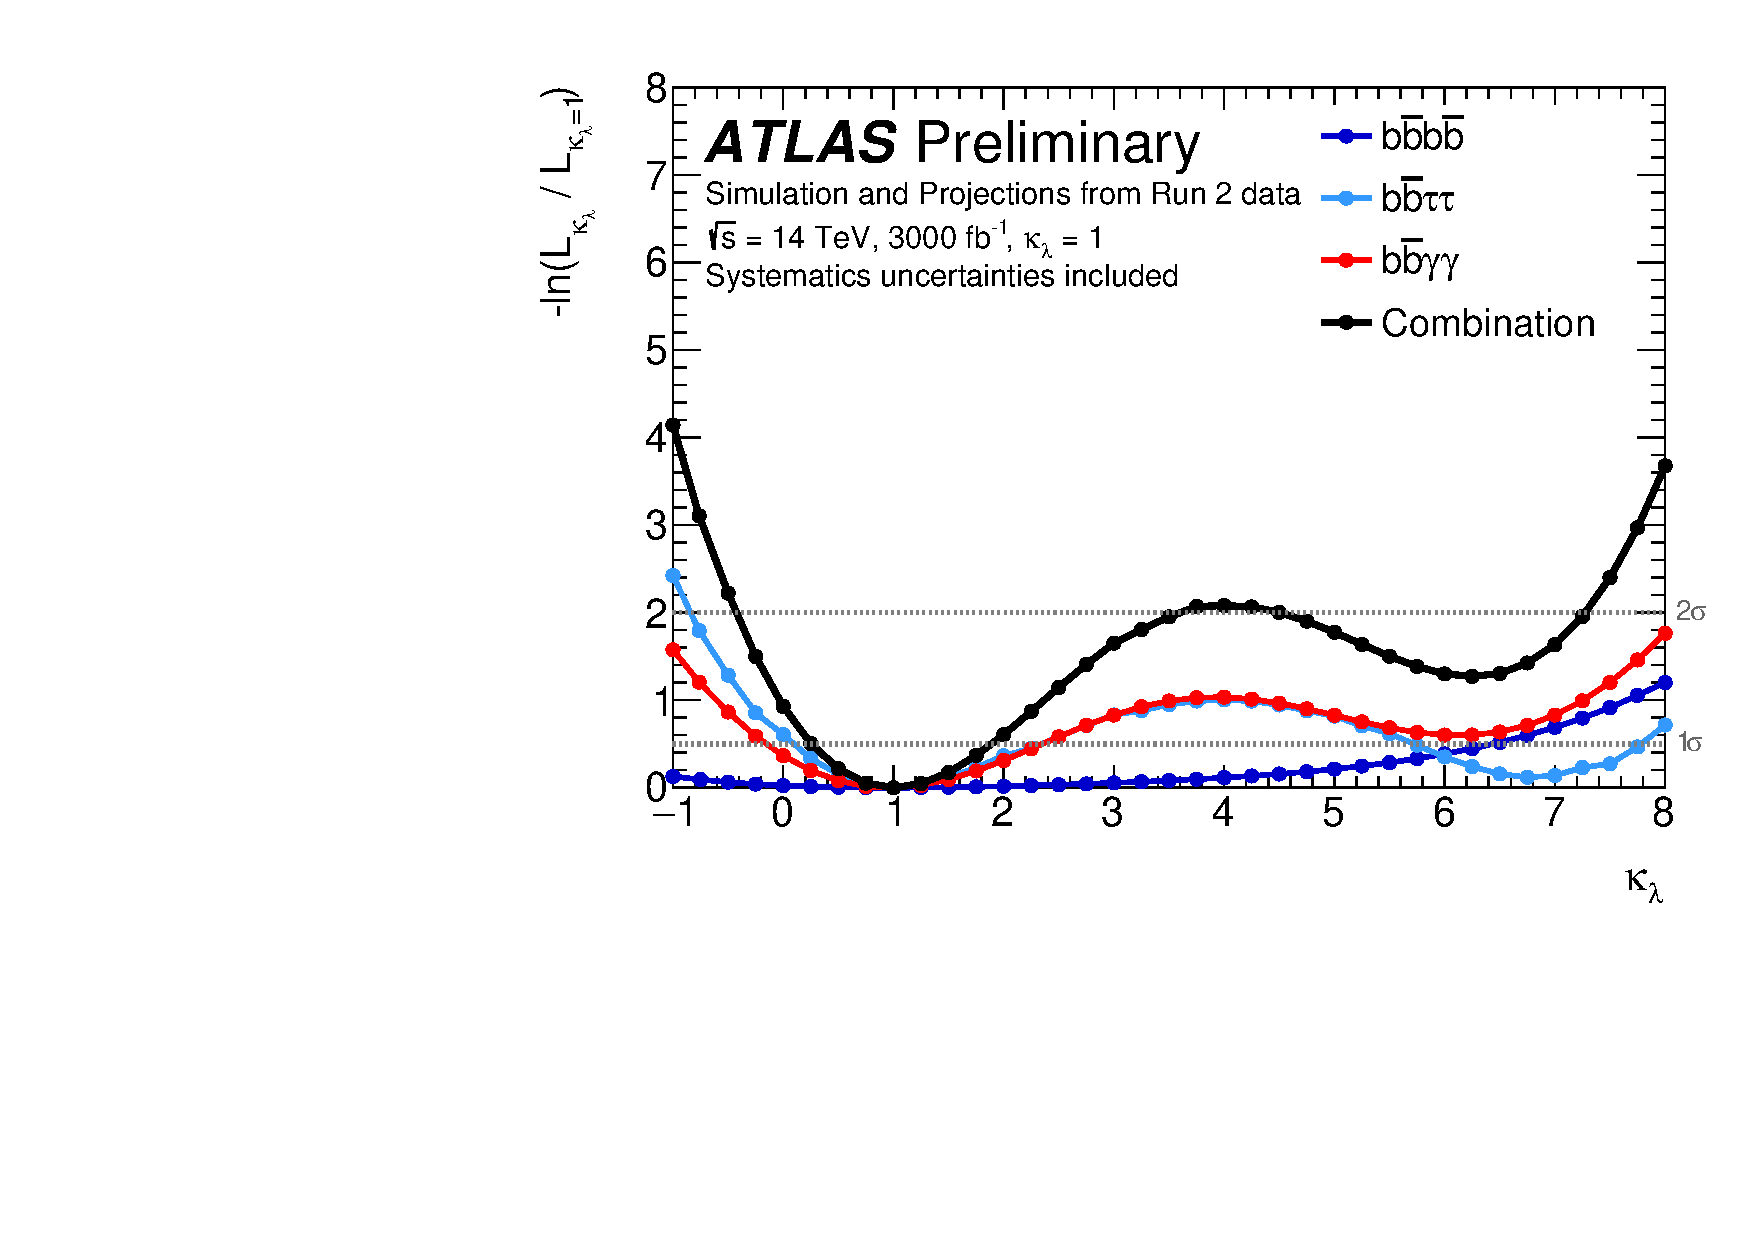
\includegraphics[width=0.5\textwidth]{\main/section3/plots/bbbb_bbtt_bbyy_lHHH0100_AllSyst_overlay_Preliminary.pdf}} 
\caption{Maximum likelihood for $\kappa_{\lambda}$ divided by the maximum likelihood for $\kappa_{\lambda}$ = 1 for (a) the fits with only statistical uncertainties and (b) the fits with all systematic uncertainties as nuisance parameters. The black circles show the results for the combination, while the coloured markers show the values coming from the individual channels. The dashed lines at $-\ln\left(L_{\kappa_{\lambda}}/L_{\kappa_{\lambda}=1}\right) = 0.5$ and 2.0 indicate the values corresponding to the $1\sigma$ and $2\sigma$ Confidence Intervals (CI), respectively (assuming an asymptotic $\chi^2$ distribution of the test statistic).} 
\label{fig:ATLAS_HH_comb} 
\end{figure}

The 68\% Confidence Intervals for $\kappa_{\lambda}$, from the likelihood ratio test performed on the Asimov dataset created from the backgrounds and the SM HH signal are $0.4 \leq \kl\ \leq 1.7$ and $0.25 \leq \kl\ \leq 1.9$ with and without systematic uncertainties respectively. The Confidence Intervals per channel are summarised in Table~\ref{tab:ATLAS_HH_kappalambda}. 
The Higgs boson self-coupling is constrained at 95\% confidence level (CL) to $-0.4\leq \kappa_{\lambda} \leq7.3$ ($-0.1\leq \kappa_{\lambda} \leq2.7\cup5.5\leq \kappa_{\lambda} \leq6.9$), with (without) systematic uncertainties.


\begin{table}[htb!]
\begin{center}
\begin{tabular}{lcc} \toprule
 & \textbf{Statistical-only} & \textbf{Statistical + Systematic}\\
\hline
$HH \rightarrow b\bar{b}b\bar{b}$ & $-0.4 \leq \kappa_{\lambda} \leq 4.3$ & $-2.3 \leq \kappa_{\lambda} \leq 6.4$ \\
$HH \rightarrow b\bar{b}\tau\tau$ &  $0.2 \leq \kappa_{\lambda} \leq 2.0 \cup 5.9 \leq \kappa_{\lambda} \leq 7.2$ & $0.1 \leq \kappa_{\lambda} \leq 2.3 \cup 5.7 \leq \kappa_{\lambda} \leq 7.8$ \\
$HH \rightarrow b\bar{b}\gamma\gamma$ &  $-0.1 \leq \kappa_{\lambda} \leq 2.4$ & $-0.2 \leq \kappa_{\lambda} \leq 2.5$ \\
combined &   $0.4 \leq \kappa_{\lambda} \leq 1.7$ & $0.25 \leq \kappa_{\lambda} \leq 1.9$ \\
\bottomrule
\end{tabular}
\end{center}
\caption{68\% Confidence Intervals for $\kappa_{\lambda}$, estimated for an Asimov dataset containing the backgrounds plus SM signal.}
\label{tab:ATLAS_HH_kappalambda}
\end{table}



Assuming the SM HH signal the expected exclusion significance for the \kl\ = 0 hypothesis, i.e. no Higgs self-coupling, is 1.4 and 1.8 standard deviations with and without systematic uncertainties respectively.







%The combination of the three decay channels leads to an expected significance of XX (XX)$\sigma$ including (without) systematics uncertainties~\cite{ATLASHHPUBnote}. The 95\% CL upper limit on the HH production cross-section is shown in Figure~\ref{fig:ATLAS_HH_b}. The allowed range at 95\% CL for $\kl$ including (without) systematic uncertainties is XX -- XX (XX -- XX). A measurement of \lHHH\ is also performed, improved by the use of the $m_{HH}$ shape in the $HH \rightarrow b\bar{b}b\bar{b}$ and $HH \rightarrow b\bar{b}\gamma\gamma$ analyses. 


